\section{Methodology}
\label{sec:methodology}
	
	\subsection{Measured Data}
	\label{ssec:measured-data}
	
		As a single spectrum contains overlapping information, it is necessary to determine both relevant wavelengths and the respective parameters to apply NIRS to practical problems.
		To select wavelengths and determine parameters we use an example data set, which contains $p^\m{(SOC)},p^\m{(N)},\m{pH}$ and wave reflectances of 319 wavelengths ranging from $1400 \unit{nm}$ to $2672 \unit{nm}$ by steps of $4 \unit{nm}$ for 533 samples.%citation

		We define $\Lambda$ as the set of all measured wavelengths. The reflectance $\varrho(\lambda)$ of a sample at a wavelength $\lambda \in \Lambda$ is recorded as
		\[
			-\lg \varrho(\lambda) = -\frac{\ln \varrho(\lambda)}{\ln 10}
		\]
		Figure \ref{fig:soil-spec-rnd} shows six randomly chosen soil spectra in a diagram.
		\begin{figure*}
			\centering
			% GNUPLOT: LaTeX picture with Postscript
\begingroup
  \makeatletter
  \providecommand\color[2][]{%
    \GenericError{(gnuplot) \space\space\space\@spaces}{%
      Package color not loaded in conjunction with
      terminal option `colourtext'%
    }{See the gnuplot documentation for explanation.%
    }{Either use 'blacktext' in gnuplot or load the package
      color.sty in LaTeX.}%
    \renewcommand\color[2][]{}%
  }%
  \providecommand\includegraphics[2][]{%
    \GenericError{(gnuplot) \space\space\space\@spaces}{%
      Package graphicx or graphics not loaded%
    }{See the gnuplot documentation for explanation.%
    }{The gnuplot epslatex terminal needs graphicx.sty or graphics.sty.}%
    \renewcommand\includegraphics[2][]{}%
  }%
  \providecommand\rotatebox[2]{#2}%
  \@ifundefined{ifGPcolor}{%
    \newif\ifGPcolor
    \GPcolorfalse
  }{}%
  \@ifundefined{ifGPblacktext}{%
    \newif\ifGPblacktext
    \GPblacktexttrue
  }{}%
  % define a \g@addto@macro without @ in the name:
  \let\gplgaddtomacro\g@addto@macro
  % define empty templates for all commands taking text:
  \gdef\gplbacktext{}%
  \gdef\gplfronttext{}%
  \makeatother
  \ifGPblacktext
    % no textcolor at all
    \def\colorrgb#1{}%
    \def\colorgray#1{}%
  \else
    % gray or color?
    \ifGPcolor
      \def\colorrgb#1{\color[rgb]{#1}}%
      \def\colorgray#1{\color[gray]{#1}}%
      \expandafter\def\csname LTw\endcsname{\color{white}}%
      \expandafter\def\csname LTb\endcsname{\color{black}}%
      \expandafter\def\csname LTa\endcsname{\color{black}}%
      \expandafter\def\csname LT0\endcsname{\color[rgb]{1,0,0}}%
      \expandafter\def\csname LT1\endcsname{\color[rgb]{0,1,0}}%
      \expandafter\def\csname LT2\endcsname{\color[rgb]{0,0,1}}%
      \expandafter\def\csname LT3\endcsname{\color[rgb]{1,0,1}}%
      \expandafter\def\csname LT4\endcsname{\color[rgb]{0,1,1}}%
      \expandafter\def\csname LT5\endcsname{\color[rgb]{1,1,0}}%
      \expandafter\def\csname LT6\endcsname{\color[rgb]{0,0,0}}%
      \expandafter\def\csname LT7\endcsname{\color[rgb]{1,0.3,0}}%
      \expandafter\def\csname LT8\endcsname{\color[rgb]{0.5,0.5,0.5}}%
    \else
      % gray
      \def\colorrgb#1{\color{black}}%
      \def\colorgray#1{\color[gray]{#1}}%
      \expandafter\def\csname LTw\endcsname{\color{white}}%
      \expandafter\def\csname LTb\endcsname{\color{black}}%
      \expandafter\def\csname LTa\endcsname{\color{black}}%
      \expandafter\def\csname LT0\endcsname{\color{black}}%
      \expandafter\def\csname LT1\endcsname{\color{black}}%
      \expandafter\def\csname LT2\endcsname{\color{black}}%
      \expandafter\def\csname LT3\endcsname{\color{black}}%
      \expandafter\def\csname LT4\endcsname{\color{black}}%
      \expandafter\def\csname LT5\endcsname{\color{black}}%
      \expandafter\def\csname LT6\endcsname{\color{black}}%
      \expandafter\def\csname LT7\endcsname{\color{black}}%
      \expandafter\def\csname LT8\endcsname{\color{black}}%
    \fi
  \fi
  \setlength{\unitlength}{0.0500bp}%
  \begin{picture}(7936.00,3400.00)%
    \gplgaddtomacro\gplbacktext{%
      \csname LTb\endcsname%
      \put(1078,704){\makebox(0,0)[r]{\strut{} 0.3}}%
      \put(1078,1190){\makebox(0,0)[r]{\strut{} 0.35}}%
      \put(1078,1676){\makebox(0,0)[r]{\strut{} 0.4}}%
      \put(1078,2163){\makebox(0,0)[r]{\strut{} 0.45}}%
      \put(1078,2649){\makebox(0,0)[r]{\strut{} 0.5}}%
      \put(1078,3135){\makebox(0,0)[r]{\strut{} 0.55}}%
      \put(1353,484){\makebox(0,0){\strut{} 1400}}%
      \put(2304,484){\makebox(0,0){\strut{} 1600}}%
      \put(3256,484){\makebox(0,0){\strut{} 1800}}%
      \put(4208,484){\makebox(0,0){\strut{} 2000}}%
      \put(5160,484){\makebox(0,0){\strut{} 2200}}%
      \put(6111,484){\makebox(0,0){\strut{} 2400}}%
      \put(7063,484){\makebox(0,0){\strut{} 2600}}%
      \put(176,1919){\rotatebox{-270}{\makebox(0,0){\strut{}$-\lg \varrho(\lambda)$}}}%
      \put(4374,154){\makebox(0,0){\strut{}$\lambda \ [\m{nm}]$}}%
    }%
    \gplgaddtomacro\gplfronttext{%
    }%
    \gplbacktext
    \put(0,0){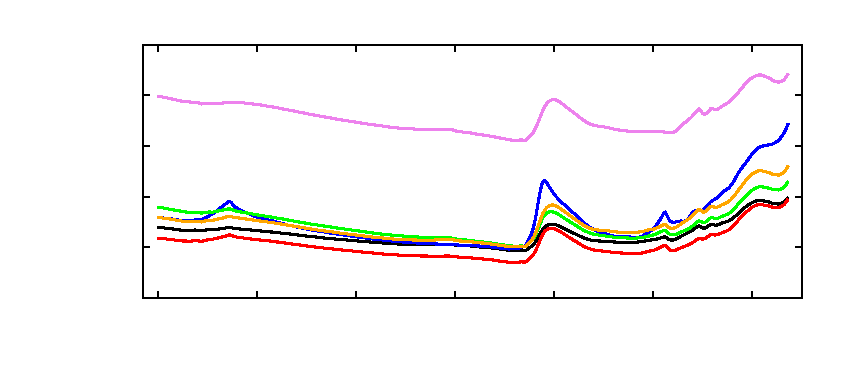
\includegraphics{gp/soil-spec-rnd}}%
    \gplfronttext
  \end{picture}%
\endgroup

			\caption{Six near infrared soil spectra of randomly chosen soil samples obtained from the data set, where $\lambda$ is the wavelength and $\rho(\lambda)$ the corresponding reflectance and each colour refers to one sample}
			\label{fig:soil-spec-rnd}
		\end{figure*}
		
	
	% subsection measured-data

	\subsection{Statistical Model}
	\label{ssec:statistical-model}
	
		Let $n\in\SN$ be the size of the data set and $k\in\SN$ with $k\leq n$ the number of measured wavelengths. We define
		$\varrho_i$ as the soil spectrum of the $i$th sample for every $i\in\SN,i\leq n$.
		$\lambda_j$ is the $j$th measured wavelength for every $j\in\SN,j\leq k$. We will alternatively refer to these as predictors.%note that we might have to introduce the term predictor at this point
		Then according to section \ref{ssec:measured-data} the measured reflectance values are $x_{ij}$ with
		\[
			x_{ij} \define -\lg \varrho_i(\lambda_j)
		\]
		for every $i,j\in\SN,i\leq n,j\leq k$.
		
	
		We define the measured ASF of $\m{SOC}$ of the $i$th sample for every $i\in\SN,i\leq n$ as $p^\m{(SOC)}_i$ to which we will also refer to as response variable.
		To simplify notation, we then define the $n$-dimensional vector
%		\begin{alignat*}{3}
		\[
			p^\m{(SOC)} \define \curvb{p^\m{(SOC)}_i}
		\]
			%p^\m{(N)} &\define&&\ \curvb{p^\m{(N)}_i} \\
			%\m{pH} &\define&&\ \curvb{\m{pH}_i}
%		\end{alignat*}

		The Beer-Lambert law allows us to make assumptions on the relations between soil spectra and the response variable.
		We saw in section \ref{ssec:nirs} that the logarithmised reflectance can be written as a linear combination of molar concentrations.
		Hence, it seems plausible to assume that an ASF can be represented by a linear combination of logarithmised reflectance values.

		Now let $P^\m{(SOC)}$ be the appropriate random vector to $p^\m{(SOC)}$.
		Then under the above assumption the expected values are given for all $i \in \SN, i \leq n$ by
		\[
			\expect P_i^\m{(SOC)} \define \beta^\m{(SOC)}_0 + \sum_{j = 1}^k{x_{ij}\beta^\m{(SOC)}_j} 
		\]
		which simplifies with an $\mathbb{X} \in \SR^{n \times (k+1)}$, called design matrix, and a parameter vector $\beta^\m{(SOC)} \in \SR^{k+1}$ to
		\[
			\expect P^\m{(SOC)} = \mathbb{X}\beta^\m{(SOC)}
		\]
		
		To capture the stochastic part of $P^\m{(SOC)}$, we extend the model to
		\begin{alignat*}{3}
			&P^\m{(SOC)} = \mathbb{X}\beta^\m{(SOC)} + \varepsilon^\m{(SOC)} \\
			&\expect \varepsilon^\m{(SOC)} = 0, \qquad \cov \varepsilon^\m{(SOC)} = (\sigma^2)^\m{(SOC)} \idmat
		\end{alignat*}
		where $(\sigma^2)^\m{(SOC)} \in (0,\infty)$. Following common practice in physics and chemistry, we further assume that 
		\[
			\varepsilon^\m{(SOC)} \sim \FN \curvb{0,(\sigma^2)^\m{(SOC)}\idmat}
		\]
		This results in the complete model
		\[
			P^\m{(SOC)} \sim \FN \curvb{\mathbb{X}\beta^\m{(SOC)},(\sigma^2)^\m{(SOC)} \idmat}
		\]
		The model for the second response variable $P^\m{(N)}$ is constructed in analogy.
		
		The case for the $\m{pH}$ is slightly different, though. 
		When modelling the corresponding random variable we have to adjust the model as the $\m{pH}$ is a logarithmised molar concentration.
		We therefore have to include this into the expected value of the corresponding random variables
		
		\[
			\expect \m{\overline{pH}}_i \define \beta^\m{\m{(pH)}}_0 + \sum_{j = 1}^k{\ln (x_{ij}) \beta^\m{(pH)}_j} 
		\]
		and denote the corresponding matrix by $\mathbb{X}_{\ln}$.

	
	% subsection statistical-model

	\subsection{Multivariate Linear Regression}
	\label{ssec:mlr}
	
		Multiple linear regression (MLR) or multivariate linear regression is a statistical method for estimating parameters of linear relations between a response variable and a set of predictors and to use these to predict new responses.
		Let $\mathbb{X}\in\SR^{n\times(k+1)}, n,k\in\SN,k<n$ be the design matrix, $\sigma^2\in(0,\infty)$ and $Y$ be the random vector variables with
		\[
			Y \sim \FN\curvb{\mathbb{X}\beta,\sigma^2\idmat_n}
		\]
		for a certain $\beta\in\SR^{k+1}$
		Then through the maximum-likelihood-method and a correction we get two best unbiased estimators $\hat{\beta},\hat{\sigma}^2$ for $\beta$ and $\sigma^2$
		\begin{alignat*}{3}
			\hat{\beta}(Y) &=&&\ \inv{\curvb{\transp{\mathbb{X}}\mathbb{X}}}\transp{\mathbb{X}}Y \\
			\hat{\sigma}^2(Y) &=&&\ \frac{1}{n-(k+1)}\norm{Y - \mathbb{X}\hat{\beta}(Y)}^2
		\end{alignat*}
		Now let $y \define (y_i)\in\SR^n$ be a realization of $Y$.
		Then we define
		\begin{alignat*}{3}
			\hat{y} &\define&&\ \mathbb{X}\hat{\beta}(y) = \mathbb{X}\inv{\curvb{\transp{\mathbb{X}}\mathbb{X}}}\transp{\mathbb{X}}y \\
			\hat{\sigma}^2 &\define&&\ \hat{\sigma}^2(y)
		\end{alignat*}
		%citation
	
	% subsection mlr

	\subsection{Mallows' $C_\m{p}$}
	\label{ssec:mallows-C_p}
	
		At this point, the model is specified using $k+1 = 320$ predictors for each response variable, using the whole measured spectra for each soil sample.
		\textbf{[this is wrong]} We know from \ref{ssec:nirs} that the light waves contain redundant information.
		This might lead to overfitting, i.e. the variance of our estimated parameters $\hat{\beta}_i(Y)$ might be too large, compromising their usability for future measurements.
		To address this problem, it is sensible to limit each actual model to a \enquote{good} subset of the predictors. Hence, our task becomes to select the best or at least a \enquote{sufficiently} good model $M$ defined by
		\[
			M\subset \Lambda \cup \set{\lambda_0}
		\]
		where $\lambda_0$ stands for the intercept.
		We denote the design matrix for each $M$ by $\mathbb{X}^{(M)}$.
		Applying MLR to the new design matrix yields the new estimators
		\begin{alignat*}{3}
			\hat{\beta}^{(M)}(Y) &=&&\ \inv{\curvb{\transp{\mathbb{X}^{(M)}}\mathbb{X}^{(M)}}}\transp{\mathbb{X}^{(M)}}Y \\
			\curvb{\hat{\sigma}^2}^{(M)}(Y) &=&&\ \frac{1}{n-\m{p}}\norm{Y - \mathbb{X}^{(M)}\hat{\beta}^{(M)}(Y)}^2,
		\end{alignat*}
		where $\m{p} \in \set{2,\ldots,k}$ corresponds to the number of predictors included in $M$.
		%to follow the logic of our argumentation, we should start with the SPSE
		
		To determine the \enquote{goodness} of $M$, we use Mallow's $C_\m{p}$ given by
		\[
			C_\m{p}^{(M)} \define \frac{1}{\hat{\sigma}^2}\sum_{i=1}^n\curvb{y_i-\hat{y}^{(M)}_i}^2 - n + 2\m{p}
		\]
		The minimization this value is equivalent to the minimization of the sum of predicted squared errors (SPSE).
	
	% subsection mallows-C_p

	\subsection{Selecting A Model}
	\label{ssec:model-selec}
	
	As the set of predictors is comparatively large, $n-k < k$, the full-sized model might overfit the data and hence lower the confidence in our parameter estimator.
	The proposed solution in \ref{mallows-C_p} is to reduce the number of predictors.
	Still, with a size of the hypothesis space of $\abs{\s{H}} = 2^{319}$, complete search or even best $k$ approaches are beyond feasibility.
	To reduce the time spent on model search, we will compare two \textsl{do we?} model selection algorithms, simulated annealing and bidirectional elimination.

		\subsubsection{Simulated Annealing}
		\label{sssec:simulated-annealing}
	
			%The set of predictors contains $k=319$ free selectable elements (the constant shall remain).
			%Therefore the power set $\s{H}$, the set of possible subsets $M$, contains of $2^{k}=2^{319}$ elements.
			We want to find a subset $M$ such that for all $N\in\s{H}$ the inequality
			\[
				C_\m{p}^{(M)} \leq C_\m{p}^{(N)}
			\]
			holds.

			Simulated annealing (SANN) is a probabilistic technique for approximating the global optimum of a given function.
			Specifically, it is a metaheuristic to approximate global optimisation in large search spaces.
			It simulates the slow cooling of a thermodynamic system through random numbers.
			With this algorithm it is possible to find a \enquote{good} local minimum in a short time.
			% Quelle: https://en.wikipedia.org/wiki/Simulated_annealing

			The algorithm is applicable to arbitrary sets, in our case $\s{H}$.
			Let $x_0\in\s{H}$ be the initial set of predictors, $T_0\in(0,\infty)$ be the initial temperature of the system and $i_\m{max}\in\SN$ be the maximal number of time steps.
			Then the algorithm requires the following functions:
			\begin{itemize}
				\item $\func{\m{cost}}{\s{H}}{\SR}$ \\
					Calculates the cost of a given predictor set.
				\item $\func{\m{temp}}{\SR\times\SN^2}{(0,\infty)}$\\
					Calculates the temperature according to the given initial temperature and time steps.
					It is a monotonically decreasing function in the second parameter.
				\item $\func{\m{nbr}}{\s{H}}{\s{H}}$ \\
					Generates a random neighbor of a given predictor set.
				\item $\func{\m{prob}}{\SR^2\times(0,\infty)}{[0,1]}$ \\
					Calculates the probability of changing the current set or state to the neighbor.
				\item $\m{rnd}(0,1)$ \\
					Returns a random number in the interval $[0,1]$.
			\end{itemize}
			The listing shows one variant of the pseudocode of the SANN algorithm. 

			\medskip
			\begin{tcolorbox}[colframe=black,colbacktitle=white,coltitle=black, attach boxed title to top center={yshift=-2mm},enhanced, titlerule=0.1pt, boxrule=0.5pt, arc=5pt,title=Listing:\quad SANN algorithm]
				\begin{tabbing}
	\qquad\=\qquad\=\qquad\=\qquad\=\kill
	$c_0 = \m{cost}(x_0)$\\
	\\
	\textbf{for} ($i=1$, $i\leq i_\m{max}$) \{\\
		\>$T = \m{temp}(T_0,i,i_\m{max})$\\
		\\
		\>$x_1 = \m{nbr}(x_0)$\\
		\>$c_1 = \m{cost}(x_1)$\\
		\\
		\>\textbf{if} $(\m{prob}(c_0, c_1, T) \geq \m{rnd}(0,1))$ \{\\
			\>\>$x_0 = x_1$\\
			\>\>$c_0 = c_1$\\
		\>\}\\
	\}
\end{tabbing}
			\end{tcolorbox}
			\medskip

	
		% subsubsection simulated-annealing
		
		\subsubsection{Bidirectional Elimination}

	\subsection{Model Validation}
	\label{ssec:model-validation}
	
		% goodness of prediction
	
	% subsection model-validation

% section methodology